% Generated by tools/paper/render.py from main_text.py; edit the source there, not this file.
\section{Results}

\subsection{Experimental setup}

Benchmarks ran on an Intel Core i9-7900X at 3.3~GHz (Skylake-X, AVX-512, ten cores) with turbo boost and hyper-threading disabled and 91~GB of memory, under Ubuntu Linux. sporos, simd-minimizers, minimap2, copMEM2 and strobealign were compiled for the native instruction set, minibwa with its default build, and MUMmer4, Mumemto, BWA and ropebwt3 were installed from Bioconda. The genome pairs were \emph{Escherichia coli} K-12 MG1655 and O157:H7 Sakai \citep{Blattner1997,Hayashi2001}, human (GRCh38 \citep{Schneider2017}) and chimpanzee (Clint \citep{Yoo2025}) chromosome 21, and GRCh38 and T2T-CHM13 \citep{Nurk2022} chromosome 1. Reads were simulated from GRCh38 chromosome 21: 1{,}000,000 of 150~bp and 4{,}000 of 10~kbp, each base replaced by a random base with probability 0.002 and half of the reads reverse-complemented. Unless stated otherwise, each command was run three times (once if it exceeded 60~s) after the machine became idle, and the best wall time is reported; MEM and SMEM tools wrote their output to files, except ropebwt3, whose output was discarded. Supplementary Section S1 lists versions and commands.

\subsection{Minimizers and syncmers}

On one thread, sporos computed minimizers and closed syncmers 1.8--2.3 times faster than simd-minimizers across all schemes on CHM13 chromosome 1 and on random DNA (Table~\ref{tab:seeds}; Supplementary Table S2); canonical (21, 11)-minimizers of chromosome 1 took 1.11~ns per base (0.90 Gbp/s). With 8 lanes, the vector width of simd-minimizers, sporos was 1.3--1.7 times faster on chromosome 1, and the 16-lane AVX-512 build was another 1.27--1.48 times faster, whereas simd-minimizers reported a slowdown with AVX-512 \citep{GrootKoerkamp2025simd}. minimap2's \texttt{mm\_sketch} was 15 times slower than sporos. On ten threads, sporos was between 1.1 times slower and 1.6 times faster than simd-minimizers; our harness for simd-minimizers only counts each thread's positions, whereas sporos returns one ordered list.

% Generated by tools/paper/render.py from main_text.py; edit the source there, not this file.
\begin{table*}[t]
\caption{Minimizers and closed syncmers of CHM13 chr1 (248~Mbp): ns per base, the best of 5 to 7 runs on one thread and of 3 on ten. Every tool reads its input already encoded (simd-minimizers packed at two bits per base, sporos at one byte per base, minimap2's mm\_sketch in ASCII) and writes positions to memory. sporos runs 16 lanes of 32 bits (AVX-512) or 8 (the width simd-minimizers uses, AVX2). mm\_sketch computes canonical minimizers only, of k at most 28 (the k = 31 rows run k = 28). Bold: fastest at each thread count.}\label{tab:seeds}
\centering\footnotesize
\setlength{\tabcolsep}{4pt}
\resizebox{\ifdim\width>\textwidth\textwidth\else\width\fi}{!}{\begin{tabular}{@{}llrrrrrrr@{}}
\toprule
 &  & \multicolumn{4}{c}{One thread} & \multicolumn{3}{c}{Ten threads} \\ \cmidrule(lr){3-6}\cmidrule(lr){7-9}
Scheme & k, w & sporos-16 & sporos-8 & simd-min. & mm\_sketch & sporos-16 & simd-min. & mm\_sketch \\
\midrule
Minimizers, forward & 21, 11 & \textbf{1.04} & 1.33 & 1.81 & -- & 0.259 & \textbf{0.192} & -- \\
Minimizers, canonical & 21, 11 & \textbf{1.02} & 1.44 & 2.17 & 17.1 & 0.268 & \textbf{0.206} & 1.97 \\
Closed syncmers, forward & 21, 11 & \textbf{1.14} & 1.45 & 2.00 & -- & \textbf{0.183} & 0.197 & -- \\
Closed syncmers, canonical & 21, 11 & \textbf{1.16} & 1.58 & 2.57 & -- & \textbf{0.180} & 0.248 & -- \\
Minimizers, forward & 31, 19 & \textbf{0.926} & 1.24 & 1.62 & -- & \textbf{0.125} & 0.156 & -- \\
Minimizers, canonical & 31, 19 & \textbf{0.923} & 1.34 & 1.91 & 15.3 & \textbf{0.138} & 0.189 & 1.92 \\
Closed syncmers, forward & 31, 19 & \textbf{0.992} & 1.31 & 1.85 & -- & \textbf{0.136} & 0.174 & -- \\
Closed syncmers, canonical & 31, 19 & \textbf{1.01} & 1.46 & 2.33 & -- & \textbf{0.135} & 0.225 & -- \\
\bottomrule
\end{tabular}}
\end{table*}


\subsection{Seed-index lookups}

Seeding 150~bp reads and looking up their minimizers, sporos processed 136~Mbp per second on one thread, 3.9 times the throughput of minimap2 (34.6~Mbp/s) for the same minimizers and occurrence cap, and 9.3 times that of strobealign for its randstrobes (Table~\ref{tab:lookups}). With one read per call, sporos remained 1.4 times faster than minimap2.

% Generated by tools/paper/render.py from main_text.py; edit the source there, not this file.
\begin{table}[t]
\caption{Seed-index lookups of 1 M simulated 150~bp reads against hg38 chr21 on one thread: throughput in Mbp of reads per second, the best of three runs, reads in memory, timing only the loop that seeds each read and copies out its hits; index build time on 1 and 8 threads. sporos and minimap2 index the same (w, k)-minimizers under different hashes and skip seeds with more than 20 hits; strobealign indexes randstrobes with its defaults for 150~bp reads and does more per seed (both orientations, partial-strobe lookups), so its rows are a reference point. minimap2's and strobealign's build times include reading the FASTA file.}\label{tab:lookups}
\centering\footnotesize
\setlength{\tabcolsep}{4pt}
\resizebox{\linewidth}{!}{\begin{tabular}{@{}lrrr@{}}
\toprule
Seeding & Mbp/s & Hits per read & Build (s), 1 / 8 threads \\
\midrule
sporos, batch (k = 19, w = 12) & \textbf{136} & 27.7 & 0.338 / 0.0645 \\
sporos, one read per call (k = 19, w = 12) & 47.0 & 27.7 &  \\
minimap2 (k = 19, w = 12) & 34.6 & 27.6 & 1.64 / 1.22 \\
sporos, batch (k = 21, w = 11) & \textbf{131} & 29.0 & 0.357 / 0.0675 \\
sporos, one read per call (k = 21, w = 11) & 46.4 & 29.0 &  \\
minimap2 (k = 21, w = 11) & 32.6 & 29.1 & 1.66 / 1.25 \\
strobealign, one hit per seed & 14.7 & 51.0 & 1.77 / 1.33 \\
strobealign, every position & 13.1 & 97.2 &  \\
\bottomrule
\end{tabular}}
\end{table}


\subsection{MEMs and MUMs}

On one thread, sporos found all MEMs of the three genome pairs 2.0--16 times faster than copMEM2, and 2.0--2.4 times faster on the chromosome 1 pair (Table~\ref{tab:mems}; Supplementary Table S3). As neither copMEM2 nor MUMmer4 divides a single query sequence among threads, sporos was 9.7--12 times faster than copMEM2 on ten threads, finding the 65.6 million MEMs of at least 50~bp between the chromosomes 1 in 3.74~s. sporos was 4.2--43 times faster than MUMmer4 for MEMs, MUMs and reference-unique MEMs (Supplementary Table S4); the smallest margin was for MUMs of the chromosome 1 pair, for which sporos first enumerates all 65.6 million MEMs. All 60 output checks passed: the outputs of sporos equalled those of MUMmer4 and copMEM2, and its ten-thread outputs its one-thread outputs. Peak memory on chromosome 1 was at most 3.5~GB (Supplementary Table S5).

% Generated by tools/paper/render.py from main_text.py; edit the source there, not this file.
\begin{table*}[t]
\caption{MEMs and MUMs of at least 50~bp between whole chromosomes, forward strand: wall time in seconds, the best of three runs (one run past 60~s), output written to a file. copMEM2 is the faster of its default and \texttt{-mf} settings; it and MUMmer4 gain nothing from more threads on a single query sequence (Supplementary Section S1). Every sporos output equals MUMmer4's, and its MEMs equal copMEM2's. Bold: fastest at each thread count.}\label{tab:mems}
\centering\footnotesize
\setlength{\tabcolsep}{4pt}
\resizebox{\ifdim\width>\textwidth\textwidth\else\width\fi}{!}{\begin{tabular}{@{}lrrrrrrrr@{}}
\toprule
 & \multicolumn{5}{c}{MEMs (\texttt{-maxmatch})} & \multicolumn{3}{c}{MUMs (\texttt{-mum})} \\ \cmidrule(lr){2-6}\cmidrule(lr){7-9}
Pair & sporos, 1 thr. & sporos, 10 thr. & copMEM2, 1 thr. & copMEM2, 10 thr. & MUMmer4 & sporos, 1 thr. & sporos, 10 thr. & MUMmer4 \\
\midrule
E. coli (4.6 / 5.5~Mbp) & \textbf{0.09} & \textbf{0.05} & 0.89 & 0.89 & 1.97 & \textbf{0.09} & 0.05 & 1.71 \\
Human / chimpanzee chr21 (47 / 33~Mbp) & \textbf{0.72} & \textbf{0.23} & 1.95 & 1.95 & 17.5 & \textbf{0.73} & 0.25 & 14.6 \\
hg38 / CHM13 chr1 (249 / 248~Mbp) & \textbf{19.5} & \textbf{3.74} & 46.3 & 46.4 & 159 & \textbf{21.0} & 3.97 & 87.5 \\
\bottomrule
\end{tabular}}
\end{table*}


\subsection{Frequency-capped MEMs}

sporos computed frequency-capped MEMs 121--176 times faster than Mumemto on one thread, using 8--18\% of its memory (Table~\ref{tab:capped}). The definitions differ, so the comparison is between the closest settings: Mumemto treats both genomes as one collection, counts occurrences on both strands and considers a match maximal if its occurrences cannot all be extended together, whereas sporos reports MUMmer-style position pairs of the query against the reference and counts occurrences in the reference as given. On the \emph{E. coli} pair, sporos reported 89--99\% of the forward-strand position pairs of Mumemto, and Mumemto 97--100\% of those of sporos. On chromosome 21 these shares were 32--93\% and 77--93\%, which we attribute to the two notions of maximality: in repeats, two copies of a string that is maximal across the collection can extend further as a pair, and sporos then reports the longer match.

% Generated by tools/paper/render.py from main_text.py; edit the source there, not this file.
\begin{table*}[t]
\caption{Frequency-capped MEMs of at least 50~bp on both strands: wall time in seconds and peak memory in MB. Mumemto (one thread) finds the multi-MEMs of the two genomes as one collection, capped per genome (\texttt{-k 2 -f N}) or in total (\texttt{-k 2 -f 0 -F N}); sporos finds the MEMs of the query against the reference whose string occurs at most N times in the reference (\texttt{-maxmatch -{}-max-occ N}, for the total cap) or in the reference and the query (\texttt{-mum -{}-max-occ N}, per genome). The definitions differ (Section 4.5): the last column gives the share of Mumemto's forward-strand position pairs that sporos also reports, and of sporos's that Mumemto reports.}\label{tab:capped}
\centering\footnotesize
\setlength{\tabcolsep}{4pt}
\resizebox{\ifdim\width>\textwidth\textwidth\else\width\fi}{!}{\begin{tabular}{@{}lrrrrrrr@{}}
\toprule
Pair and cap & sporos, 1 thr. & sporos, 10 thr. & Mumemto & Speedup & sporos MB & Mumemto MB & Shared (\%) \\
\midrule
E. coli, at most 3 per genome & \textbf{0.11} & 0.06 & 13.3 & 121 & 61 & 348 & 97 / 99 \\
E. coli, at most 10 per genome & \textbf{0.11} & 0.06 & 13.3 & 121 & 61 & 348 & 89 / 100 \\
E. coli, at most 3 in total & \textbf{0.10} & 0.05 & 13.3 & 133 & 61 & 348 & 99 / 97 \\
E. coli, at most 10 in total & \textbf{0.10} & 0.06 & 13.3 & 133 & 61 & 348 & 94 / 99 \\
chr21, at most 3 per genome & \textbf{1.02} & 0.31 & 169 & 166 & 257 & 3{,}130 & 77 / 93 \\
chr21, at most 10 per genome & \textbf{1.05} & 0.33 & 170 & 162 & 257 & 3{,}130 & 32 / 88 \\
chr21, at most 3 in total & \textbf{0.96} & 0.28 & 169 & 176 & 257 & 3{,}130 & 93 / 83 \\
chr21, at most 10 in total & \textbf{0.98} & 0.28 & 170 & 174 & 257 & 3{,}130 & 54 / 77 \\
\bottomrule
\end{tabular}}
\end{table*}


\subsection{SMEMs and f-SMEMs}

On one thread, sporos found the SMEMs of 150~bp reads 4.8 times faster than minibwa, 15 times faster than \texttt{bwa fastmap} and 51 times faster than ropebwt3 without position output, and those of 10~kbp reads 5.7, 17 and 65 times faster (Table~\ref{tab:smems}). For f-SMEMs, sporos was 2.3 times faster than minibwa at f = 2 and 2.3 times at f = 5, and 32 and 29 times faster than ropebwt3. Requiring two occurrences slowed the search 4.2 times relative to SMEMs, since a match that occurs once no longer ends it. sporos and \texttt{bwa fastmap} differed in 20 of 1.22 million SMEMs of the short reads; all 14 reported only by BWA pass through an N of the reference, which BWA replaces with random bases (Supplementary Section S3). Ten threads gave the same SMEMs as one.

% Generated by tools/paper/render.py from main_text.py; edit the source there, not this file.
\begin{table*}[t]
\caption{SMEMs (f = 1) and f-SMEMs of at least 19~bp of simulated reads against hg38 chr21, both strands: wall time in seconds, the best of three runs, the index loaded from disk. sporos, minibwa and bwa fastmap list the positions of SMEMs with at most 20 hits; ropebwt3 is run without positions, its default, which favours it. minibwa and bwa fastmap are single-threaded; bwa computes no f-SMEMs. Bold: fastest at each thread count.}\label{tab:smems}
\centering\footnotesize
\setlength{\tabcolsep}{4pt}
\resizebox{\ifdim\width>\textwidth\textwidth\else\width\fi}{!}{\begin{tabular}{@{}lrrrrrr@{}}
\toprule
 & \multicolumn{4}{c}{One thread} & \multicolumn{2}{c}{Ten threads} \\ \cmidrule(lr){2-5}\cmidrule(lr){6-7}
Reads & sporos & minibwa & bwa & ropebwt3 & sporos & ropebwt3 \\
\midrule
1 M reads of 150~bp, SMEMs & \textbf{1.85} & 8.95 & 27.5 & 93.5 & \textbf{0.40} & 9.64 \\
1 M reads of 150~bp, f = 2 & \textbf{7.79} & 17.6 & -- & 246 & \textbf{1.09} & 24.9 \\
1 M reads of 150~bp, f = 5 & \textbf{7.51} & 17.5 & -- & 216 & \textbf{1.10} & 21.9 \\
4{,}000 reads of 10~kbp, SMEMs & \textbf{0.37} & 2.11 & 6.37 & 24.1 & \textbf{0.14} & 2.49 \\
4{,}000 reads of 10~kbp, f = 2 & \textbf{2.45} & 5.36 & -- & 73.8 & \textbf{0.41} & 7.51 \\
4{,}000 reads of 10~kbp, f = 5 & \textbf{2.41} & 5.40 & -- & 65.0 & \textbf{0.39} & 6.64 \\
\bottomrule
\end{tabular}}
\end{table*}


% Generated by tools/paper/render.py from main_text.py; edit the source there, not this file.
\begin{figure}[t]
\centering
\resizebox{\linewidth}{!}{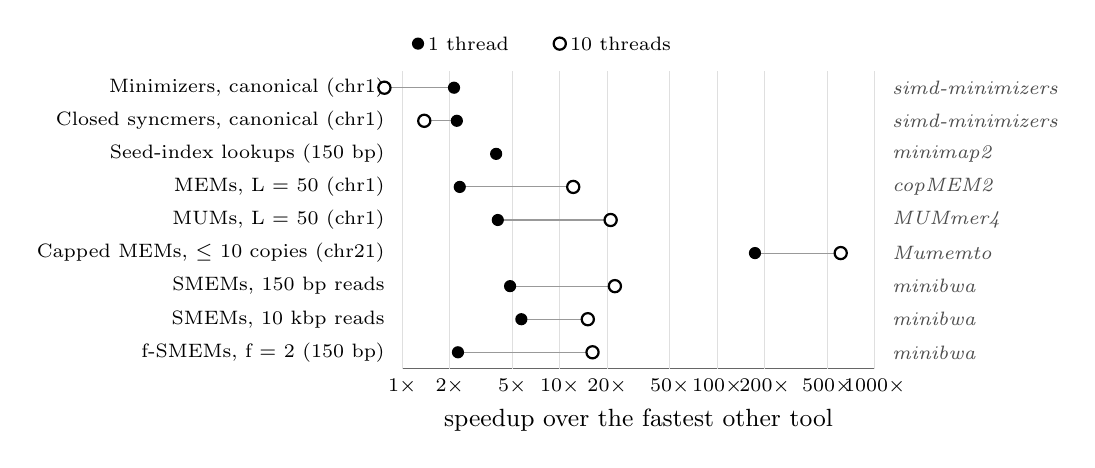
\begin{tikzpicture}
\draw[black!60] (0,0) -- (6.0,0);
\draw[gray!25] (0.000,0) -- (0.000,3.780);\node[below, font=\scriptsize] at (0.000,0) {1$\times$};
\draw[gray!25] (0.602,0) -- (0.602,3.780);\node[below, font=\scriptsize] at (0.602,0) {2$\times$};
\draw[gray!25] (1.398,0) -- (1.398,3.780);\node[below, font=\scriptsize] at (1.398,0) {5$\times$};
\draw[gray!25] (2.000,0) -- (2.000,3.780);\node[below, font=\scriptsize] at (2.000,0) {10$\times$};
\draw[gray!25] (2.602,0) -- (2.602,3.780);\node[below, font=\scriptsize] at (2.602,0) {20$\times$};
\draw[gray!25] (3.398,0) -- (3.398,3.780);\node[below, font=\scriptsize] at (3.398,0) {50$\times$};
\draw[gray!25] (4.000,0) -- (4.000,3.780);\node[below, font=\scriptsize] at (4.000,0) {100$\times$};
\draw[gray!25] (4.602,0) -- (4.602,3.780);\node[below, font=\scriptsize] at (4.602,0) {200$\times$};
\draw[gray!25] (5.398,0) -- (5.398,3.780);\node[below, font=\scriptsize] at (5.398,0) {500$\times$};
\draw[gray!25] (6.000,0) -- (6.000,3.780);\node[below, font=\scriptsize] at (6.000,0) {1000$\times$};
\node[font=\small] at (3.00,-0.65) {speedup over the fastest other tool};
\node[anchor=east, font=\scriptsize] at (-0.10,3.570) {Minimizers, canonical (chr1)};
\node[anchor=west, font=\scriptsize\itshape, black!70] at (6.10,3.570) {simd-minimizers};
\draw[black!40] (-0.227,3.570) -- (0.657,3.570);
\fill[black] (0.657,3.570) circle (2.2pt);
\draw[black, fill=white, thick] (-0.227,3.570) circle (2.2pt);
\node[anchor=east, font=\scriptsize] at (-0.10,3.150) {Closed syncmers, canonical (chr1)};
\node[anchor=west, font=\scriptsize\itshape, black!70] at (6.10,3.150) {simd-minimizers};
\draw[black!40] (0.279,3.150) -- (0.693,3.150);
\fill[black] (0.693,3.150) circle (2.2pt);
\draw[black, fill=white, thick] (0.279,3.150) circle (2.2pt);
\node[anchor=east, font=\scriptsize] at (-0.10,2.730) {Seed-index lookups (150 bp)};
\node[anchor=west, font=\scriptsize\itshape, black!70] at (6.10,2.730) {minimap2};
\fill[black] (1.192,2.730) circle (2.2pt);
\node[anchor=east, font=\scriptsize] at (-0.10,2.310) {MEMs, L = 50 (chr1)};
\node[anchor=west, font=\scriptsize\itshape, black!70] at (6.10,2.310) {copMEM2};
\draw[black!40] (0.730,2.310) -- (2.171,2.310);
\fill[black] (0.730,2.310) circle (2.2pt);
\draw[black, fill=white, thick] (2.171,2.310) circle (2.2pt);
\node[anchor=east, font=\scriptsize] at (-0.10,1.890) {MUMs, L = 50 (chr1)};
\node[anchor=west, font=\scriptsize\itshape, black!70] at (6.10,1.890) {MUMmer4};
\draw[black!40] (1.213,1.890) -- (2.646,1.890);
\fill[black] (1.213,1.890) circle (2.2pt);
\draw[black, fill=white, thick] (2.646,1.890) circle (2.2pt);
\node[anchor=east, font=\scriptsize] at (-0.10,1.470) {Capped MEMs, $\le$ 10 copies (chr21)};
\node[anchor=west, font=\scriptsize\itshape, black!70] at (6.10,1.470) {Mumemto};
\draw[black!40] (4.479,1.470) -- (5.568,1.470);
\fill[black] (4.479,1.470) circle (2.2pt);
\draw[black, fill=white, thick] (5.568,1.470) circle (2.2pt);
\node[anchor=east, font=\scriptsize] at (-0.10,1.050) {SMEMs, 150 bp reads};
\node[anchor=west, font=\scriptsize\itshape, black!70] at (6.10,1.050) {minibwa};
\draw[black!40] (1.369,1.050) -- (2.700,1.050);
\fill[black] (1.369,1.050) circle (2.2pt);
\draw[black, fill=white, thick] (2.700,1.050) circle (2.2pt);
\node[anchor=east, font=\scriptsize] at (-0.10,0.630) {SMEMs, 10 kbp reads};
\node[anchor=west, font=\scriptsize\itshape, black!70] at (6.10,0.630) {minibwa};
\draw[black!40] (1.512,0.630) -- (2.356,0.630);
\fill[black] (1.512,0.630) circle (2.2pt);
\draw[black, fill=white, thick] (2.356,0.630) circle (2.2pt);
\node[anchor=east, font=\scriptsize] at (-0.10,0.210) {f-SMEMs, f = 2 (150 bp)};
\node[anchor=west, font=\scriptsize\itshape, black!70] at (6.10,0.210) {minibwa};
\draw[black!40] (0.707,0.210) -- (2.416,0.210);
\fill[black] (0.707,0.210) circle (2.2pt);
\draw[black, fill=white, thick] (2.416,0.210) circle (2.2pt);
\fill[black] (0.2,4.130) circle (2.2pt) node[right, font=\scriptsize] {1 thread};\draw[black, fill=white, thick] (2.0,4.130) circle (2.2pt) node[right, font=\scriptsize] {10 threads};
\end{tikzpicture}}
\caption{Speedup of sporos over the fastest other tool for each task, on one thread (filled) and ten (hollow), each tool at its best on that many threads; the other tool is named on the right (Tables 1 to 5). copMEM2, MUMmer4, minibwa, bwa fastmap and Mumemto use one thread; the seed-lookup harnesses run one.}\label{fig:speedups}
\end{figure}

